\chapter{Geometry}

Pixels in the image plane have a direct mapping to the position of the camera in the real world. When we use the approximation of the image we might lose some relevant pieces of information such as the depth of the objects in the scene or the speed of objects, which will appear slower the further they are from the camera. 
\\
In this chapter we will introduce the basic concepts of geometry that will allow us to understand the relationship between the camera and the real world.
\\
Typically, we represent a point (pixel) as a set of coordinates:

\[ P = [ x, y ]^t = \begin{bmatrix} x \\ y \end{bmatrix}\]
Often is convenient to use homogeneous coordinates:
\[ P = [ x, y ]^t = [sx, sy, s]\]
Where \( s \) is a scaling factor, commonly set to 1.0, this will help us when doing transformations.

\[ P = [ x, y ]^t = [x, y, 1]\]
Sometimes we can also omit the " \(^t\) " and write the coordinates as a row vector.

\section{Affine Transformations}

Now formally the pixel is a vector so in general we can apply all the kind of transformations we want, which usually turn out to be combinations of summations and multiplications. 
The most common transformations are:

\begin{itemize} 
    \item Scaling 
    \item Translation 
    \item Rotation 
    \item Combinations of the above 
\end{itemize}

\subsection{Scaling}

In scaling we take one point or a set of points and we transform them by a multiplying factor. 

\[
\begin{bmatrix}
    x' \\
    y'
    \end{bmatrix}
    =
    \begin{bmatrix}
    c & 0 \\
    0 & c
    \end{bmatrix}
    \begin{bmatrix}
    x \\
    y
    \end{bmatrix}
\]

\begin{figure}[ht]
    \centering
    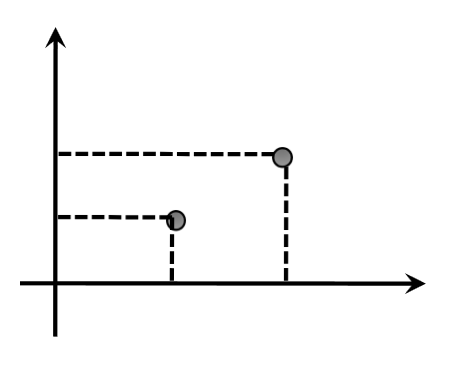
\includegraphics[width=0.3\textwidth]{Figures/scaling.png}
    \caption{Scaling}
    \label{fig:scaling}
\end{figure}

This is a very simple transformation, it can happen that we have not a single coefficient \(c\) but different scaling factors for the different axis.
\[
\begin{bmatrix}
    x' \\
    y'
    \end{bmatrix}
    =
    \begin{bmatrix}
    c_x & 0 \\
    0 & c_y
    \end{bmatrix}
    \begin{bmatrix}
    x \\
    y
    \end{bmatrix}
\]

\subsection{Rotation}

Rotation is the result of applying a rotation angle to the coordinate points, if we go back to the trigonometry we can see that we can use the sine and cosine information of the angle \(\theta\) and we can imagine that if we are rotating a unit vector, the coordinates of the new vector will be the sine and cosine of the angle.
\\\\\\
\begin{figure}[ht]
    \centering
    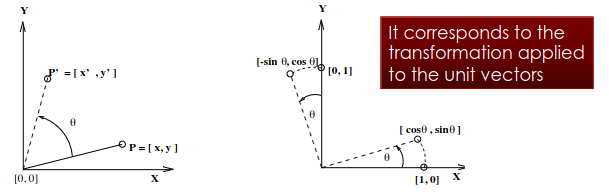
\includegraphics[width=0.75\textwidth]{Figures/rotation.png}
    \caption{Rotation}
    \label{fig:rotation}
\end{figure}

For instance, we can see on the horizontal unit vector how the \(x\) gets reduced while a \(y\) component appears corresponding to the sine of the angle.
\\
By the time we have a point that's been shifter by a certain amount \(\theta\), saying that the points rotates equals to keeping the point fixed and rotating the coordinate system by the same amount. The resulting operation that we have in our matrix is the multiplication of the point with the transformation of the unit vectors.

\[
    \begin{bmatrix}
        x' \\
        y'
        \end{bmatrix}
        =
        \begin{bmatrix}
        \cos\theta & -\sin\theta \\
        \sin\theta & \cos\theta
        \end{bmatrix}
        \begin{bmatrix}
        x \\
        y
        \end{bmatrix}
        =
        \begin{bmatrix}
        x \cos\theta - y \sin\theta \\
        x \sin\theta + y \cos\theta
        \end{bmatrix}    
\]
\\
Both scaling and rotation can be constructed using a simple 2 by 2 matrix.
\subsection{Translation}

A translation is simply a shift of the points of our objects into new coordinates.
Just like we can think of rotation as a change in the coordinate system, we can think of translation as a change in the origin of the coordinate system.
\\
If we apply a displacement vector it's the same as moving the origin of the coordinate system to the new point and we can model this easily:

\(\quad \quad \quad \quad \quad \quad \quad \quad \quad \quad \quad \quad D([x, y]) = [x + x_0, y + y_0] \)
\\
At this point we can't use anymore a 2 by 2 matrix because we have to introduce the two operators \( x_0 \) and \( y_0 \) that are not part of the matrix. 

\[
    \begin{bmatrix}
        x' \\
        y' \\
        \end{bmatrix}
        =
        \begin{bmatrix}
        1 & 0  \\
        0 & 1  \\
        \end{bmatrix}
        \begin{bmatrix}
        x \\
        y \\
        \end{bmatrix}
        +
        \begin{bmatrix}
            x_0 \\
            y_0 \\
        \end{bmatrix}
\]
\\
The new coordinates are nothing but a multiplication of a scaling matrix of factor 1.0 by the coordinates \(x, y\) and then the addition of the translation vector.
\\
To bring the displacement vector inside the matrix we can use the homogeneous coordinates, we can add a third coordinate to the vector and then we can multiply the matrix by the vector.

\[
    \begin{bmatrix}
        x' \\
        y' \\
        1
        \end{bmatrix}
        =
        \begin{bmatrix}
        1 & 0 & x_0 \\
        0 & 1 & y_0 \\
        0 & 0 & 1
        \end{bmatrix}
        \begin{bmatrix}
        x \\
        y \\
        1
        \end{bmatrix}
        =
        \begin{bmatrix}
        x + x_0 \\
        y + y_0 \\
        1
        \end{bmatrix}
\]


\subsection{Rotation, scaling and translation}

Our goal is to be able to map what's happening in the real world to the image plane, we can do this by applying a series of transformations, overall we need to deal with at least 4 parameters:
\begin{itemize} 
    \item One rotation angle (1 parameter)
    \item One scaling factor (1 parameter)
    \item A translation vector (2 parameters)
\end{itemize}

\[{}^w P_j = D_{x0,y0} S_s R_\theta {}^i P_i\]
\\
We can describe this combination of transformations with the formula above, where \(D_{x0,y0}\) is the translation matrix, \(S_s\) is the scaling matrix, \(R_\theta\) is the rotation matrix, \(w\) is the world coordinates, \(i\) is the image coordinates and \(j\) a generic point.

\begin{figure}[H]
    \centering
    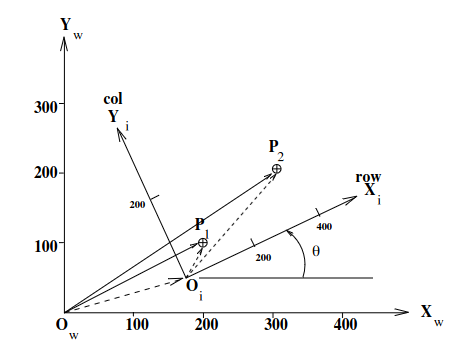
\includegraphics[scale = 0.6]{Figures/comb.png}
    \caption{Here we are applying a translation, a rotation and a scaling to the point \(P\)}
    \label{fig:comb}
\end{figure}

We can write the formula above as a matrix multiplication:

\[
    \begin{bmatrix}
    x_w \\
    y_w \\
    1
    \end{bmatrix}
    =
    \begin{bmatrix}
    1 & 0 & x_0 \\
    0 & 1 & y_0 \\
    0 & 0 & 1
    \end{bmatrix}
    \begin{bmatrix}
        s & 0 & 0 \\
        0 & s & 0 \\
        0 & 0 & 1
    \end{bmatrix}
    \begin{bmatrix}
    \cos\theta & -\sin\theta & 0 \\
    \sin\theta & \cos\theta & 0 \\
    0 & 0 & 1
    \end{bmatrix}
    \begin{bmatrix}
        x \\
        y \\
        1
    \end{bmatrix}
\]
\\
So to obtain the transformation matrix we need to solve a system of equations with 4 unknowns, the 4 parameters we mentioned before. To obtain 4 equations we can use 2 points called control points (obtaining \(x_1, y_1\) and \(x_2, y_2\)), such points must be clearly visible both in the image and in the real world planes. Once we have found these two points we are able to map these coordinates on the image plane.
\\
We keep referring to the transformations in Figure \ref{fig:comb} as \(2D \rightarrow 2D \) transformations, this implies we have a ground plane on which we are working on and a camera plane, the camera plane is the image plane that might be scaled, translated with respect to the ground plane. At the moment we are not considering a rotation of the camera, we are assuming the image plane is parallel to the ground plane.

\begin{figure}[H]
    \centering
    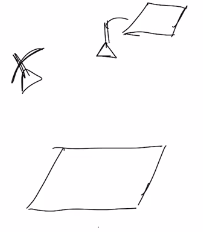
\includegraphics[width=0.2\textwidth]{Figures/planes.png}
    \caption{The camera plane we are considering now is parallel to the ground plane}
    \label{fig:planes}
\end{figure}

\subsection{General Affine Transformations}

Starting from the previous transformations we can see that the 3 matrices are of the same size and if we compute the product between all of them we can think of these transformations as an end-to-end transformation where we can embed all these parameters in a single matrix.

\[
    \begin{bmatrix}
    u \\
    v \\
    1
    \end{bmatrix}
    =
    \begin{bmatrix}
    a_{11} & a_{12} & a_{13} \\
    a_{21} & a_{22} & a_{23} \\
    0 & 0 & 1
    \end{bmatrix}
    \begin{bmatrix}
        x \\
        y \\
        1
    \end{bmatrix}
\]

This transformation is the set of coefficients, we don't know exactly the contribution of each of the 3 matrices, but it results in a certain transformation which is represented by what is called in general the \textbf{Camera Matrix}. It tells us exactly how to move from a certain plane where \(x, y\) lie to where they will be in the camera plane, and vice versa.
\\
We see that we have 6 coefficients instead of the 4 parameters, to determine them it's the same as we did before, with the exception that instead of 2 we need 3 matching control points for which we know the position of in the real world and in the image plane. However, finding these points might now be trivial,
the main difficulty is being precise in picking them.
\\
What is usually done is, instead of using the minimum required control points, picking up more points with the hope that on average we are making a very small mistake, averaging out the errors. This way we might end up with 12, 20 equations and 6 unknowns (an \textit{over-determined system}), our goal is to find the 6 equations that minimize the error. We use the \textit{least-squares method} to find the best solution that minimizes the error.
\[
    \varepsilon (a_{11}, a_{12}, a_{13}, a_{21}, a_{22}, a_{23}) = 
\sum_{j=1}^{n} (a_{11}x_j + a_{12}y_j + a_{13} - u_j)^2 
+ (a_{21}x_j + a_{22}y_j + a_{23} - v_j)^2
\]

What we are trying to get is to find the best configuration of these coefficients in a way that the difference between what's expected from the transformation and what's observed is minimized. The resulting equation system is:

\[
    \begin{bmatrix}
        \sum x^2_j & \sum x_jy_j & \sum x_j & 0 & 0 & 0 \\
        \sum x_jy_j & \sum y^2_j & \sum y_j & 0 & 0 & 0 \\
        0 & 0 & 0 & \sum x^2_j & \sum x_jy_j & \sum x_j \\
        0 & 0 & 0 & \sum x_jy_j & \sum y^2_j & \sum y_j \\
        0 & 0 & 0 & \sum x_j & \sum y_j & \sum 1 
    \end{bmatrix}
    \begin{bmatrix}
        a_{11} \\
        a_{12} \\
        a_{13} \\
        a_{21} \\
        a_{22} \\
        a_{23}
    \end{bmatrix}
    =
    \begin{bmatrix}
        \sum x_ju_j \\
        \sum y_ju_j \\
        \sum u_j \\
        \sum x_jv_j \\
        \sum y_jv_j \\
        \sum v_j
    \end{bmatrix}
\]

The solution is found by computing the minimum of the error, or in other terms compute the \textit{partial derivative} with respect to each unknown and set them to zero, making sure the error between the result of the transformation and the observed points is minimized.

And this is how the whole thing works, how we determine the \textbf{2D camera matrix} used to map the real world plane to the camera plane. Remember that we are talking about two different planes one on top of the other, we don't have full 3D rotations \textit{yet}.

\section{Going 3D}

We are now moving to more general solutions, we can't expect from the system we'll take in consideration to end up in the easy scenario where the two planes are parallel and facing each other.
More in general what happens is that the image plane we are dealing with is something that results from a generic camera prospective where what we see in the image plane is something that look more like shown in Figure \ref{fig:3d}.

\begin{figure}[h!]
    \centering
    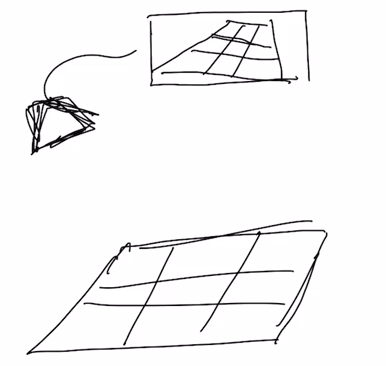
\includegraphics[width=0.2\textwidth]{Figures/3d.png}
    \caption{A generic 3D scenario.}
    \label{fig:3d}
\end{figure}

We need to go through a process called \textbf{calibration} where we'll need to determine the so called \textbf{intrinsic} and \textbf{extrinsic} parameters of the camera. The projections that we have seen so far won't be enough to describe the 3D world, we'll need to add an \textit{additional view} to make possible to determine the unique 3D coordinates \(X Y Z\) that are necessary to describe the position of a point in the real world. 
\\With that additional information we can do many tasks:
\begin{itemize} 
    \item Point Clouds
    \item Structure From Motion
    \item Mesh Reconstruction
\end{itemize}

\subsection{Intrinsic and Extrinsic Parameters}

\begin{itemize} 
    \item\textit{Intrinsic parameters} refer to the specific characteristics of the camera, such as the focal length, the distortion of the lens, the position of the principal point, etc. These parameters are fixed and don't change with the position of the camera. They are necessary because we want to link the pixel coordinates with the corresponding coordinates in the camera coordinates system.

    \item\textit{Extrinsic parameters} refer to the position of the camera in the real world, such as the rotation and translation of the camera with respect to the world coordinates. These parameters are not fixed and change with the position of the camera.
\end{itemize}

When we try to estimate these parameters we go through a process called \textbf{calibration}, where we try to find a suitable matrix which helps us to map the points in the real world to what we see through the camera.

\subsection{3D Affine Transformations}

At this point we need to go through the transformations that we have seen in the 2D case, extending them by adding a new dimension. The main difference is that our starting point is a set of 3D coordinates.
\[ [P_x, P_y, P_z] \rightarrow  [sP_x, sP_y, sP_z, s] \]
Also in this case we move from a 3D vector to a 4D vector with the addition of the scaling factor of the homogeneous coordinates.
\\
Now we have a system for each camera so a triplet of coordinates for Camera 1 and a triplet of coordinates for Camera 2, these two cameras are looking at the world coordinates, in some cases it could be interesting to also know the coordinates of the model in the world (although it's not common). 
\\We end up with:
\begin{itemize} 
    \item Model coordinates
    \item World coordinates
    \item Camera 1 coordinates
    \item Camera 2 coordinates
\end{itemize}

\begin{figure}[H]
    \centering
    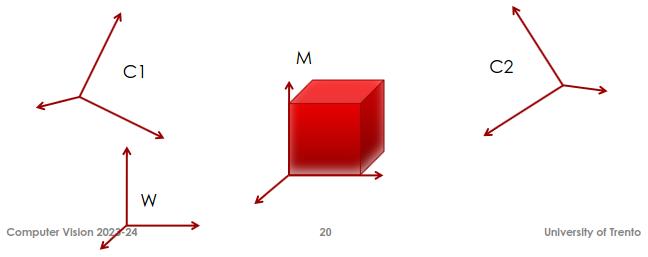
\includegraphics[width=0.8\textwidth]{Figures/coo.png}
    \caption{The new model with two camera views.}
    \label{fig:coo}
\end{figure}

We can see all these 4 systems linked by a transformation, which is nothing more than a rotation-translation to go from any of the 3 systems to the others. At the end it means that we need to deal with a rotation matrix and a translation vector.
\({}^wP = T R {}^mP\) and same for \({}^1P\) and \({}^2P\).
\\Where T is a translation vector and R a rotation matrix. It must be noted that the point seen from the first camera might be different from the second camera, both in terms of coordinates and in the sense that Camera 1 and Camera 2 might have opposite views, meaning that there might be no one-to-one mapping of all points. If there's a superset of points that's visible from both cameras, we'll be able to reconstruct the 3D position only for the points visible from both cameras.
\\\\\textit{NB: The notation for the next section will be \({}^kP_j\) where \(k\) is the camera number and \(j\) is the point number.}

\subsection{3D Translation}

Across the two views in order to move the point from a camera to the other we apply a translation,
it consists of applying a translation \(x_0, y_0, z_0\) to the point and no scaling.

\[
    {}^2P = T(x_0, y_0, z_0) {}^1P 
\]

\[
    \begin{bmatrix}
        {}^2P_x \\
        {}^2P_y \\
        {}^2P_z \\
        1
    \end{bmatrix}
    =
    \begin{bmatrix}
        1 & 0 & 0 & x_0 \\
        0 & 1 & 0 & y_0 \\
        0 & 0 & 1 & z_0 \\
        0 & 0 & 0 & 1
    \end{bmatrix}
    \begin{bmatrix}
        {}^1P_x \\
        {}^1P_y \\
        {}^1P_z \\
        1
    \end{bmatrix}   
\]

\subsection{3D Scaling}

Here, similarly to the previous case, we can have different scaling factors, although usually we have the same scaling factor for all the axis.

\[
  {}^2P = S(s_x, s_y, s_z) {}^1P 
\]

\[
    \begin{bmatrix}
        {}^2P_x \\
        {}^2P_y \\
        {}^2P_z \\
        1
    \end{bmatrix}
    =
    \begin{bmatrix}
        s_x & 0 & 0 & 0 \\
        0 & s_y & 0 & 0 \\
        0 & 0 & s_z & 0 \\
        0 & 0 & 0 & 1
    \end{bmatrix}
    \begin{bmatrix}
        {}^1P_x \\
        {}^1P_y \\
        {}^1P_z \\
        1
    \end{bmatrix}   
\]

\subsection{3D Rotation}

In terms of rotation, things become a little more complicated, we don't have a single rotation (in the 2D space we have to deal with a single angle) but since now we have an additional axis we have a rotation around the three axis, if we want to do the same analysis as we did in the 2D case with the unit vector we end up with three matrices of coefficients that describe the rotation around each of the three axis.

\begin{multicols}{2}

    

\[
  {}^2P = R(X, \varTheta ) {}^1P 
\]

\[
    \begin{bmatrix}
        {}^2P_x \\
        {}^2P_y \\
        {}^2P_z \\
        1
    \end{bmatrix}
    =
    \begin{bmatrix}
        1 & 0 & 0 & 0 \\
        0 & \cos\theta & -\sin\theta & 0 \\
        0 & \sin\theta & \cos\theta & 0 \\
        0 & 0 & 0 & 1
    \end{bmatrix}
    \begin{bmatrix}
        {}^1P_x \\
        {}^1P_y \\
        {}^1P_z \\
        1
    \end{bmatrix}   
\]

\[
  {}^2P = R(Y, \varTheta ) {}^1P 
\]

\[
    \begin{bmatrix}
        {}^2P_x \\
        {}^2P_y \\
        {}^2P_z \\
        1
    \end{bmatrix}
    =
    \begin{bmatrix}
        \cos\theta & 0 & \sin\theta & 0 \\
        0 & 1 & 0 & 0 \\
        -\sin\theta & 0 & \cos\theta & 0 \\
        0 & 0 & 0 & 1
    \end{bmatrix}
    \begin{bmatrix}
        {}^1P_x \\
        {}^1P_y \\
        {}^1P_z \\
        1
    \end{bmatrix}   
\]
\end{multicols}
\[
  {}^2P = R(Z, \varTheta ) {}^1P 
\]

\[
    \begin{bmatrix}
        {}^2P_x \\
        {}^2P_y \\
        {}^2P_z \\
        1
    \end{bmatrix}
    =
    \begin{bmatrix}
        \cos\theta & \sin\theta & 0 & 0 \\
        -\sin\theta & \cos\theta & 0 & 0 \\
        0 & 0 & 1 & 0 \\
        0 & 0 & 0 & 1
    \end{bmatrix}
    \begin{bmatrix}
        {}^1P_x \\
        {}^1P_y \\
        {}^1P_z \\
        1
    \end{bmatrix}   
\]

\subsection{3D General Configuration}

Our goal is to then put everything together in a single matrix, this is the generic 3D affine transformation that maps a point in the 3D coordinates of the first system to the 3D coordinates of the second system.

\[
    \begin{bmatrix}
        {}^2P_x \\
        {}^2P_y \\
        {}^2P_z \\
        1
    \end{bmatrix}
    =
    \begin{bmatrix}
       r_{11} & r_{12} & r_{13} & t_x \\
       r_{21} & r_{22} & r_{23} & t_y \\
       r_{31} & r_{32} & r_{33} & t_z \\
        0 & 0 & 0 & 1
    \end{bmatrix}
    \begin{bmatrix}
        {}^1P_x \\
        {}^1P_y \\
        {}^1P_z \\
        1
    \end{bmatrix}   
\]

It's some sort of camera matrix, but at this point we are dealing with something that returns 3D coordinates and unfortunately doesn't help us much because at the end what we have is an image plane where the coordinates are only rows and columns, \(x, y\). It means that we need to further modify this matrix in order to end up with a representation that's 2D. We need to add to our transformation what are the proprieties of the camera, this gives us the opportunity to move from the 3D coordinates (in our case the world \(W\)) to a 2D plane \(I\).

\[
    {}^IP = {}^I_W C^WP
\]

This matrix here flattens the information and returns a 2D vector corresponding to the position in the rows and columns of the image plane and this happens by adopting a 3 by 4 matrix that gives us the chance to move from the 3D world to the 2D camera coordinates.

\[
    \begin{bmatrix}
        s^IP_r \\
        s^IP_c \\
        s
    \end{bmatrix}
    =
    {}^I_W C^W
    \begin{bmatrix}
        {}^WP_x \\
        {}^WP_y \\
        {}^WP_z \\
        1
    \end{bmatrix}  
    = 
    \begin{bmatrix}
        c_{11} & c_{12} & c_{13} & c_{14} \\
        c_{21} & c_{22} & c_{23} & c_{24} \\
        c_{31} & c_{32} & c_{33} & 1
    \end{bmatrix}
    \begin{bmatrix}
        {}^WP_x \\
        {}^WP_y \\
        {}^WP_z \\
        1
    \end{bmatrix}
\]

Unfortunately we are still not happy because while it's true that we have a 2D representation of the 3D world, we are not yet in the image plane, we are still in the camera coordinates (notice the capital \(P\)s in the formulation) and in the continuous space. We need to further modify this matrix to move from the camera coordinates to the image plane.

We need to rework again on these transformations moving from the camera to some additional coordinates:\\
\textit{(While important the following part till the end of the section was covered briefly)}
\[
    \begin{bmatrix}
        {}^CP_x \\
        {}^CP_y \\
        {}^CP_z \\
        1
    \end{bmatrix}
    =
    \begin{bmatrix}
       r_{11} & r_{12} & r_{13} & t_x \\
       r_{21} & r_{22} & r_{23} & t_y \\
       r_{31} & r_{32} & r_{33} & t_z \\
        0 & 0 & 0 & 1
    \end{bmatrix}
    \begin{bmatrix}
        {}^WP_x \\
        {}^WP_y \\
        {}^WP_z \\
        1
    \end{bmatrix}   
\]

\[
    {}^CP = {}^C_W TR(\alpha, \beta, \gamma, t_x, t_y, t_z) {}^WP
\]

\({}^CP\) is about the \textit{camera coordinates}, and
not the \textit{image coordinates} \({}^FP\), we need to project these on the image coordinates and successively discretize them in the pixel coordinates.

\[
    {}^FP = {}^F_C \varPi (f) {}^CP
\]

\[
    {}^FP = {}^F_C \varPi (f) TR(\alpha, \beta, \gamma, t_x, t_y, t_z) {}^WP
\]


\[
    \begin{bmatrix}
        s^FP_r \\
        s^FP_c \\
        s
    \end{bmatrix}
    =
    \begin{bmatrix}
        d_{11} & d_{12} & d_{13} & d_{14} \\
        d_{21} & d_{22} & d_{23} & d_{24} \\
        d_{31} & d_{32} & d_{33} & 1
    \end{bmatrix}
    \begin{bmatrix}
        {}^WP_x \\
        {}^WP_y \\
        {}^WP_z \\
        1
    \end{bmatrix}
\]

The conversion from mm to pixel consists of a scaling factor related to the real size of the pixels where \(d_x\) is the size of the pixel in the x direction and \(d_y\) is the size of the pixel in the y direction.

\[
  {}^IP={}^I_F S^F P  
\]


\[
    {}^I_F S^F
    = 
    \begin{bmatrix}
        0 & -1/d_y & 0\\
        1/d_x & 0 & 0\\
        0 & 0 & 1
    \end{bmatrix}
\]

The minus sign is due to the fact that the origin is usually bottom left but in the image it's top left, so we flip the coordinates.
\\
Overall in order to get the position rows and columns on the image plane we need to go from 3D generic world coordinates to the camera coordinates, then we need the intrinsic information of the camera, and then we need to discretize the pixels.

\[
  [p_r, p_c]^T = {}^IP = {}^I_F S^F_C \varPi (f)^C_W TR(\alpha, \beta, \gamma, t_x, t_y, t_z) {}^WP
\]

And we finally get out final camera matrix:

\[
    \begin{bmatrix}
        s^Ip_r \\
        s^Ip_c \\
        s
    \end{bmatrix}
    = 
    \begin{bmatrix}
        c_{11} & c_{12} & c_{13} & c_{14} \\
        c_{21} & c_{22} & c_{23} & c_{24} \\
        c_{31} & c_{32} & c_{33} & 1
    \end{bmatrix}
    \begin{bmatrix}
        {}^WP_x \\
        {}^WP_y \\
        {}^WP_z \\
        1
    \end{bmatrix}
\]

At the end the entire iter of transformations that we use to go from the 3D points in space to the pixel coordinates is included in the $3 \times 4$ camera matrix. It means that overall we need to compute 11 parameters (we are not considering the scaling parameter) and in order to create a reasonable mapping of the points we need to compute these coefficients. We'll see that the process that we follow to obtain the coefficients if basically the same as the 2D case.

\section{Calibration}

What we did till now was introducing some geometry problems by saying that what we want to do is to find the relationships between different domains: what happens in the real world and what happens on the camera side. During the process of acquisition the relationships between the two domains change through rotations, translations and scaling. To describe them we came up with a \textit{camera matrix} that helps us to map what happens in the real world with what happens in the camera.

The \(3 \times 4\) camera matrix contains 12 coefficients, 11 of which are unknown, we need to find them in order to map the points in the real world to the image plane. The process of finding these coefficients is called \textbf{calibration}.

In order to determine the 11 unknowns we need 6 matching pairs (12 equations) which are enough to solve the system. To pick them we do the same as in the simpler 2D case, we choose points in the real world for whom we know the coordinates and we choose the same points in the image plane, we need to be very precise in picking these points, so usually we pick a \textit{higher number} of points to average out the errors.

It's common to use an object of known geometry (a calibration patter) for which we know the relative position of the points and for this we compute the matching.


\subsection{Calibration Procedure}

As we have seen before, we have the points in the 3D world, we have the matching 2D projections and we can start constructing our equations system.
\\
Given a 3D point \([{}^WP_x {}^WP_y {}^WP_z]\) and its projection \([{}^IP_r {}^IP_c] = [u v]\) for each point in the calibration process we can write the system of equations:
\setcounter{MaxMatrixCols}{20}

\[
    \begin{bmatrix}
        x_j & y_j & z_j & 1 & 0 & 0 & 0 & 0 & -x_ju_j & -y_ju_j & -z_ju_j \\
        0 & 0 & 0 & 0 & x_j & y_j & z_j & 1 & -x_jv_j & -y_jv_j & -z_jv_j \\
    \end{bmatrix}
    \begin{bmatrix}
        c_{11} \\
        c_{12} \\
        c_{13} \\
        c_{14} \\
        c_{21} \\
        c_{22} \\
        c_{23} \\
        c_{24} \\
        c_{31} \\
        c_{32} \\
        c_{33} \\
    \end{bmatrix}
    =
    \begin{bmatrix}
        u_j \\
        v_j
    \end{bmatrix}
\]

As usual our goal is to rely on the least square to find the configuration of the matrix the minimizes the error between the observed points and the points that we expect from the transformation, the error between the actual image point measurements and the world points comes from.

\[
    {}^IP={}^I_WC^WP  
\]


\begin{figure}[H]
    \centering
    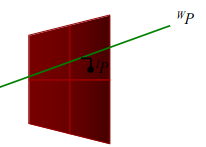
\includegraphics[width=0.4\textwidth]{Figures/proj.png}
    \caption{Error in the projection.}
    \label{fig:proj}
\end{figure}

In an ideal world all the points coming from the real world all the points are being projected in the center of projection, we can trace  the ray through the camera plane and that's it. In the real world we make mistakes, and as shown in Figure \ref{fig:proj} the points are not exactly where we expect them to be, the error is the difference between the expected and the observed points, what we are trying to do is to minimize this error.

\subsection{Computing the 3D position of a point}

Now we are in the situation where we can map points in the real world on the image plane and can get closer to one of our biggest issues: with just a single camera we cannot compute the full 3D coordinates of a point. If we add an additional camera we can have two different systems, at that point we have 4 equations (2 for each camera) and if we know the camera matrices for each camera we can come up with the 3D position of the point.
\\
Given a generic point \([x, y, z] \) and given two projections \([r_1, c_1]\) and \([r_2, c_2]\) we can write:

\begin{multicols}{2}

    \[
        \begin{bmatrix}
            sr_1 \\
            sc_1 \\
            s
        \end{bmatrix}  
        =
        \begin{bmatrix}
            b_{11} & b_{12} & b_{13} & b_{14} \\
            b_{21} & b_{22} & b_{23} & b_{24} \\
            b_{31} & b_{32} & b_{33} & 1
        \end{bmatrix}
        \begin{bmatrix}
            x \\
            y \\
            z \\
            1
        \end{bmatrix}
    \]

    \[
        \begin{bmatrix}
            tr_2 \\
            tc_2 \\
            t
        \end{bmatrix}  
        =
        \begin{bmatrix}
            c_{11} & c_{12} & c_{13} & c_{14} \\
            c_{21} & c_{22} & c_{23} & c_{24} \\
            c_{31} & c_{32} & c_{33} & 1
        \end{bmatrix}
        \begin{bmatrix}
            x \\
            y \\
            z \\
            1
        \end{bmatrix}
    \]
\end{multicols}

To compute and reconstruct the 3D position of the point we can solve the system of equations and find a solution.

If we assume that we have the projections, we know that they are subject to a certain error. That error is caused by an approximation of the projection and can be seen in the real world as a discrepancy in the intersection of the two rays.


\begin{figure}[H]
    \centering
    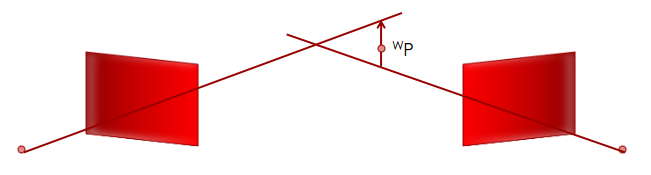
\includegraphics[width=0.7\textwidth]{Figures/inter.png}
    \caption{Error in the intersection.}
    \label{fig:inter}
\end{figure}

Usually what's done is to take the distance between the two lines and use the middle point as the 3D position of the point. 

\section{The Binocular Stereo}

As the name suggests it's basically a system that looks like Figure \ref{fig:inter} where we have two cameras and we try to come up with few equations to model that situation which, by no coincidence, is the same system humans are equipped with. It can be scaled up with multiple cameras, but the idea is the same as it becomes a pairwise binocular system anyways. 
\\The computation of the 3D position of a point usually goes through 2 steps:
\begin{itemize}
    \item Computation of the correspondences (main source of error) 
    \item Reconstruction of the 3D position (basically deterministic)
\end{itemize}

The conditions for a binocular system is that overall we have two cameras positioned anywhere in the real world pointing at a scene where there's an area that overlaps. From the area that's visible by both camera we can compute the reconstruction.

\begin{figure}[H]
    \centering
    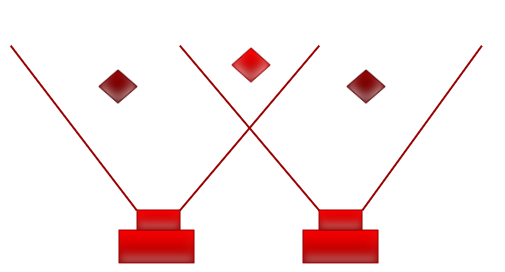
\includegraphics[width=0.6\textwidth]{Figures/binoc.png}
    \caption{This is also a specific case where both cameras are parallel and aligned (coplanar) as in most commercial stereo systems.}
    \label{fig:binoc}
\end{figure}




\begin{figure}[h!]
    \centering
    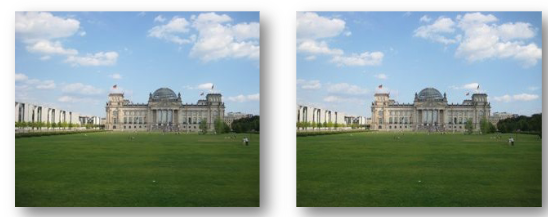
\includegraphics[width=0.6\textwidth]{Figures/coplan.png}
    \caption{Coplanar views.}
    \label{fig:coplan}
\end{figure}

In the case of coplanar cameras the difference between the views will be just a small offset as shown in Figure \ref{fig:coplan}. Points will result shifted, and the shift will depend on the depth of the point, the further the point the smaller the shift, this leads to the \textbf{parallax}, apparent motion.  

\subsection{Computing correspondences}

The first step is to compute the correspondences, in order to do so we need to find those points that are representing the same portion of the real world and this is possible mostly because if we have a good acquisition system the distance is not too big, it's normal to look for a certain match in the local area around the point of interest.

We can rely also on the \textbf{Epipolar Constraint} which tells us that the correspondences can be met along a horizontal line called the \textit{epipolar line}.

\subsection{Stereo Vision and Epipolar Geometry}

\begin{figure}[H]
    \centering
    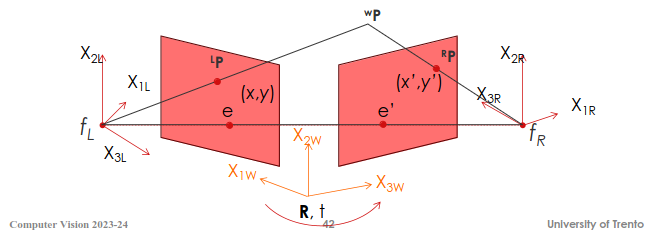
\includegraphics[width=0.75\textwidth]{Figures/stereo.png}
    \caption{A generic stereo system.}
    \label{fig:stereo}
\end{figure}

This is a slightly more complex system compared to the coplanar one. We have a Left and a Right camera, both will have their camera coordinates system and we also have to coordinates of the real world. Our objective is to start from a point available in the real world, look where the point is being projected in the first and second camera and use the information of this projection to infer the coordinates of \({}^WP\).

\[
    \begin{bmatrix}
        x \\
        y
    \end{bmatrix}
    \begin{bmatrix}
        x' \\
        y'
    \end{bmatrix}
    \rightarrow 
    \begin{bmatrix}
        X \\
        Y \\
        Z
    \end{bmatrix}
\]

We need to go through the \textbf{Epipolar Geometry}.

\begin{figure}[H]
    \centering
    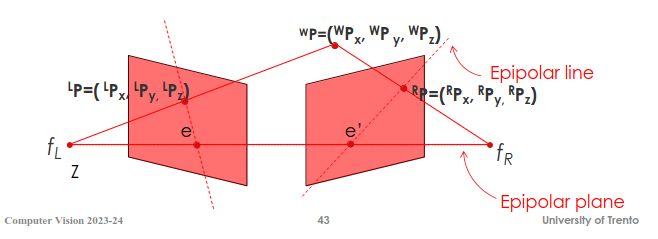
\includegraphics[width=0.75\textwidth]{Figures/epipolar.png}
    \caption{Epipolar geometry.}
    \label{fig:epipolar}
\end{figure}

The \textbf{epipolar plane} is what connects the  \({}^WP\) with the two cameras, this plane can be seen as something anchored to axis \(f_L\) and \(f_R\), since they don't move, depending on where the point is in the world what chances in the inclination of the plane. The intersection in between the epipolar plane and the image plane is what we call the \textbf{epipolar lines}. The points \(e\) and \(e'\) are the \textbf{epipoles} and they are the intersection of the epipolar lines with the image plane, they are useful because, for example, as the \({}^WP\) moves along its projection line on \(f_R\) (basically the ray that goes from \(f_R\) to \({}^WP\)) its projection on the right image plane will remain the same meanwhile its projection on the left image plane will move exclusively along the epiploar line: we \textit{know} that we only need to look in that area to find the correspondence. 

\begin{figure}[H]
    \centering
    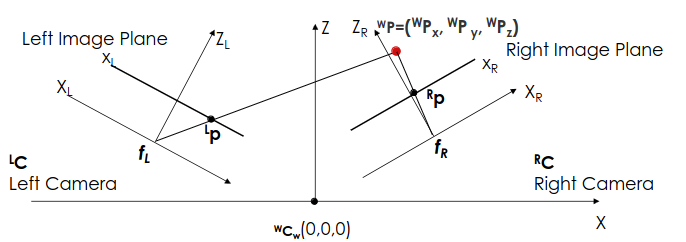
\includegraphics[width=0.75\textwidth]{Figures/epipolar_above.png}
    \caption{The same system from above.}
    \label{fig:epipolar_above}
\end{figure}

We have 


\[{}^RP = ({}^RP_x, {}^RP_y, {}^RP_z) \;\;\;\;
{}^LP = ({}^LP_x, {}^LP_y, {}^LP_z)\;\;\;\;
{}^WP = ({}^WP_x, {}^WP_y, {}^WP_z)\]


\[
    {}^RP = {}^RR{}^WP+{}^RT
\]
\[
    {}^LP = {}^LR{}^WP+{}^LT  
\]

We know that the point seen from the camera systems will be the result of a some roto-translations of the point in the real world to the coordinate system of the cameras, \(R\) and \(T\) are related to the extrinsic parameters of the cameras.

The only common term between the two last equations is \({}^WP\), so we can substitute and get:

\[
    {}^LP = {}^LR{}^RR^{-1}{}^RP-{}^LR{}^RR^{-1}{}^RT+{}^LT
\]

\[
    = M^RP+B
\]

Where the term \(M\) is a matrix that multiplies \({}^RP\), plus a term \(B\). This tells us that in between the \(L\) and the \(R\) we have a roto-translation. Using the simplified perspective projections $(Z >> f)$ we obtain the coordinates on the two image planes:

\begin{multicols}{2}

\[
    {}^Lp_x = f\frac{{}^LP_x}{{}^LP_z}  
\] 
\[
    {}^Lp_y = f\frac{{}^LP_y}{{}^LP_z}
\]

\end{multicols}

\begin{multicols}{2}

\[
    {}^Rp_x = f\frac{{}^RP_x}{{}^RP_z}  
\] 
\[
    {}^Rp_y = f\frac{{}^RP_y}{{}^RP_z}
\]
    
\end{multicols}

from which we obtain 

\[
    \frac{{}^LP_z}{f}
    \begin{bmatrix}
        {}^Lp_x \\
        {}^Lp_y \\
        f
    \end{bmatrix}
    =
    \frac{{}^RP_z}{f}
    M
    \begin{bmatrix}
        {}^Rp_x \\
        {}^Rp_y \\
        f 
    \end{bmatrix}
    + B
\]

\subsection{Estimation of the 3D position}

Some computations are not trivial, so we will see the simplified situation where the cameras are parallel and aligned. The math problem is always the same: we want to get the coordinates of \({}^WP\) given the two projections on the two image planes.

\begin{figure}[H]
\[
        \bm{{}^WP_z = \frac{fb}{{}^Lp_x-{}^Rp_x}}
\]
\caption{Formula to compute the depth of the point. \textit{It's strongly recommended memorizing this formula}.
}
\end{figure}


\begin{figure}[H]
    \centering
    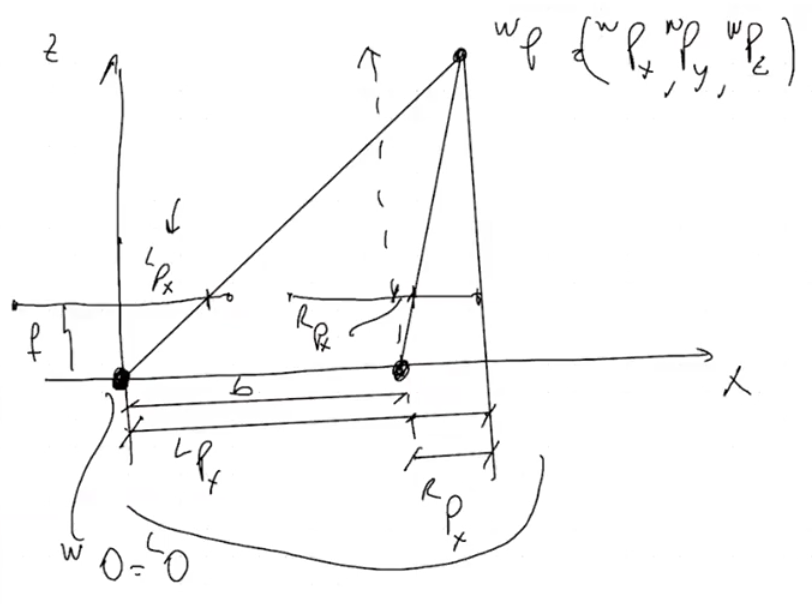
\includegraphics[width=0.75\textwidth]{Figures/epi_comp.png}
    \caption{Computations to get the depth of a point from the projections.}
    \label{fig:epi_comp}
\end{figure}

In Figure \ref{fig:epi_comp} it's shown our coplanar stereo system with focal length \(f\), \({}^WP\) is the point in the real world, the two projections on image planes are \({}^Lp_x\) and \({}^Rp_x\) and in order to complete the system we need the \({}^LP_x\) and \({}^RP_x\) which are the coordinates of the point with respect to the camera systems. 

We can say that: 

\begin{figure}[H]    
\[
    {}^Lp_x = \frac{f{}^LPx}{P_z}\;\;\;\;\;   
    {}^Rp_x = \frac{f{}^RPx}{P_z}  
\]
\caption{Projection equations.}
\label{eq:proj}
\end{figure}
Note that we are using \(P_z\) for both because the cameras are parallel and aligned, so it's the same:

\[
    {}^WP_z = {}^LP_z = {}^RP_z
\]

We put the origin of the world in the origin of one of the two cameras, this is what happens in real stereo systems. From here we can play around with equations \ref{eq:proj}:

\[
    {}^LP_x = \frac{{}^Lp_xP_z}{f}    
\]

If the cameras are distant one from the other by a certain amount \(b\) we can say (\textit{I guess \(b\) is a negative value in this example}):

\[
    {}^LP_x = b+{}^RP_x
\]

At this point we use this expression to evaluate the projection on the right camera:

\[
    {}^Rp_x = \frac{f({}^LP_x-b)}{P_z}    
\]

We know already what was our \({}^LP_x\), so we can say that: 

\[
    {}^Rp_x = \frac{f({}^LP_x-b)}{P_z}    
    =
    \frac{f({}^Lp_xPz)}{fP_z}-\frac{fb}{P_z}
\]
\[
    {}^Rp_x ={}^Lp_x-\frac{fb}{P_z}
\]
\[
    {}^Lp_x- {}^Rp_x = \frac{fb}{P_z}
\]
\[
    \bm{{P_z} = \frac{fb}{{}^Lp_x- {}^Rp_x}}
\]
Finally we have the component \(P_z\) that we have been looking for. To get to this point we have many values that play a role:
\begin{itemize}
    \item \(b\) is something that relates to the extrinsic parameters of the camera
    \item \(f\) is one of the intrinsic parameters of the camera
    \item \({}^Rp_x \;\; {}^Lp_x\) are the projections of the point in the two image planes. This term is also called the \textbf{disparity} and it's the offset between the two projections, this disparity term changes accordingly to the distance of the object from the cameras.
\end{itemize}

\begin{figure}[H]
    \centering
    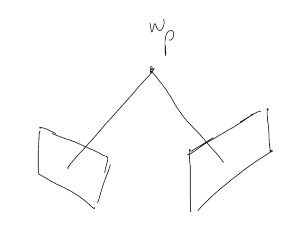
\includegraphics[width=0.4\textwidth]{Figures/mistake.png}
    \caption{Typical exam question: \textit{Please, tell how we compute the 3D coordinates of a point starting from a camera system that is parallel and aligned.} Don't draw this. Just don't.}
    \label{fig:mistake}
\end{figure}

\subsection{Matching points}

Now that we know how to get the 3 coordinates given the projections we need to understand how to compute the match, and define an evaluation function to understand how good the match is. 

The matching is usually done by looking at the intensity of the pixels, a common technique is to use \textbf{Window-based approaches}. They are very generic in computer vision, and it goes like this:

\begin{itemize}
    \item Take a window around the point of interest in the left image
    \item Along the epipolar line find the windows that best match the right and left image, shifting of a handful of pixels at a time or even pixel by pixel.
    \item Compute an error function (MSE, SAD, SSD)
    \item Find the minimum
    \item Winner-take-all and that's the \textit{disparity}. Usually we define a range of disparities, otherwise we would have to look along the entire epipolar line.
\end{itemize}

\begin{figure}[H]
    \centering
    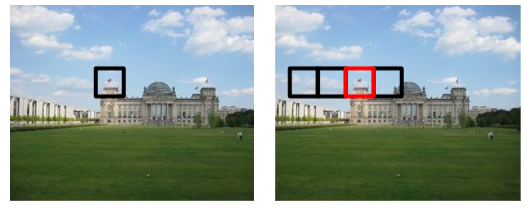
\includegraphics[width=0.6\textwidth]{Figures/sad.png}
    \caption{Moving the window along the epipolar line.}
    \label{fig:sad}
\end{figure}



\subsection{Image Normalization}

Unfortunately the two cameras are not \textit{exactly} the same, and might have small differences in the acquisition in terms of colors, even with an offset of just one or two grayscale values, our metric could become noisy, this why images get \textbf{normalized}


\begin{multicols}{2}
\[
\bar{I} = \frac{1}{|W(x,y)|} \sum_{(u,v) \in W(x,y)} I(u,v)
\]
We can compute the average value of the pixels in the window.

\end{multicols}

\begin{multicols}{2}
\[
\| I \|_{W(x,y)} = \sqrt{\sum_{(u,v) \in W(x,y)} [I(u,v) - \bar{I}]^2}
\]
Compute the window magnitude.
\end{multicols}

\begin{multicols}{2}
\[
\hat{I}(x,y) = \frac{I(x,y) - \bar{I}}{\| I - \bar{I} \|_{W(x,y)}}
\]

Calculate the normalized values, with this normalization we can eliminate the offset between the two images.
\end{multicols}

This makes it possible to compute the distance because we now know that what we have on the right side and the left side is the same. Since this normalization makes the windows comparable we can now compute the SAD or the \textbf{Sum of Squared Differences}:
\[
SSD(x,y,d) = \sum_{(u,v) \in W(x,y)} [\hat{I}_L(u,v) - \hat{I}_R(u-d,v)]^2
\]

Another metric is called the \textbf{Correlation}, a big error corresponds to small correlation and vice versa. What happens in this case is that instead of comparing the pixel to pixel values, we take the window and represent it as a vector. For instance a \(3\times 3\) window will be represented as a \(1\times9\) dimensional vector, we can then compute the correlation between the two vectors.
\[
C(d) = \frac{1}{|w-\bar{w}|}\frac{1}{|w'- \bar{w}'|}(w-\bar{w})(w'-\bar{w}')
\]
Where \(d\) represents the window shift, \(w\) and \(w'\) are the vectorized windows and \(\bar{w}\) and \(\bar{w}'\) are the averages of the vectorized windows. Basically it's a comparison between vectors where we want to measure the angle between \(w - \bar{w}\) and \(w' - \bar{w}'\).
\[
C(d) = \sum_{(u,v) \in W(x,y)} [\hat{I}(u,v) \hat{I}(u-d,v)] = w\cdot w' = \cos\theta    
\]
In the normalized case, the correlation is maximum if the original brightness of the two windows is shifted by an offset and a scale factor. This means that by the time we compute the correlation with have normalized the vectors (for instance between 0 and 1) and that the correlation is maximum when the angle between the two vectors in 0, \textit{however} it can be that the vectors are in fact, shifted and scaled, while maintaining the same angle. 

\begin{multicols}{2}
\[
\hat{I} = \lambda I + \mu
\]
\begin{figure}[H]
    \centering
    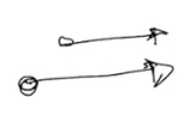
\includegraphics[width=0.1\textwidth]{Figures/vectors.png}
    \caption{Scaled and shifted vectors with maximum correlation.}
    \label{fig:vectors}
\end{figure}
\end{multicols}

Computing the correlation at each frame for the whole image
can be expensive, in practice we have windows that overlap so one of the tricks in the implementation is to keep track of the parts of the window that are common between the two windows and update the correlation accordingly. In addition, usually the correlation is carried out taking into account the disparity.

\subsection{General Stereo Configuration}

Now we want to move from the simplified stereo rig to a better characterization of a general stereo configuration, we still have our two cameras which are observing an object in the real world, we still have our \({}^WP=[{}^WP_x, {}^WP_y,{}^WP_z]\) and then we have two arbitrary cameras positioned somewhere in the real world. Again we want to find the correspondencies between the point \({}^WP\) which is seen by the camera C1 in position \({}^1P\) and by the camera C2 in position \({}^2P\).

\begin{figure}[H]
    \centering
    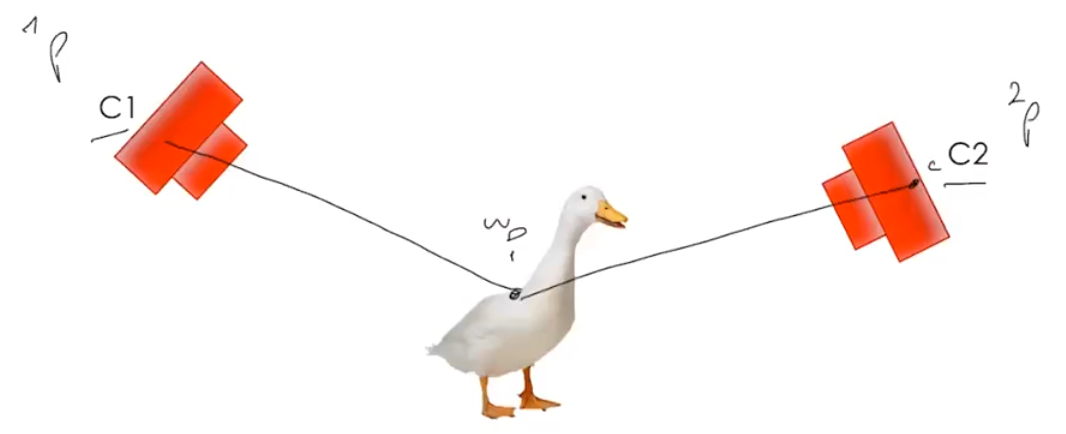
\includegraphics[width=0.65\textwidth]{Figures/duck.png}
    \caption{Quack.}
    \label{fig:duck}
\end{figure}

We know already that the two lines in Figure \ref{fig:duck} will never match exactly but we want to find the configuration that minimizes the error.


What do we need?
\begin{itemize}
\item Position of C1 and some internal parameters such as the focal
length, we know that this information is embedded in the camera matrix, which defines the relationship between the points in the real world and the image plane.
\item The same stuff for C2.
\item The corresponding matching projections of \({}^WP\) in the two image planes.
\item Finally we compute the 3D position of \({}^WP\) starting from the positions of \({}^1P\) and \({}^2P\).
\end{itemize}
\begin{figure}[H]
    \centering
    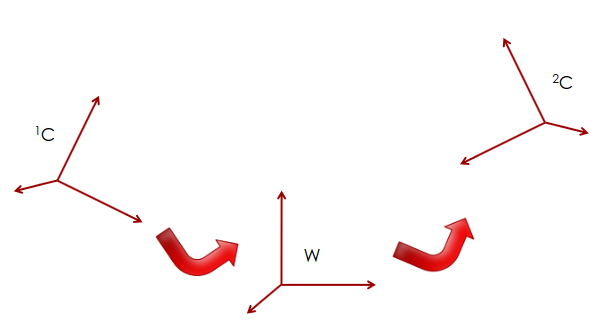
\includegraphics[width=0.65\textwidth]{Figures/world.png}
    \caption{The world is the shared information.}
    \label{fig:world}
\end{figure}

\subsection{The Fundamental Matrix}

It's the representation of the epipolar geometry in case of two generic views, it's a \(3\times3\) matrix that can map \(p\) into \(p'\) 

\[
    p' {}^TFp=0
\]

We don't need to have the intrinsic parameters, we just need to take a snapshot from the two cameras finding a set of corresponding points, and we can compute the transformation between the points in \({}^1P\) and \({}^2P\) using the fundamental matrix. 

\begin{figure}[H]
    \centering
    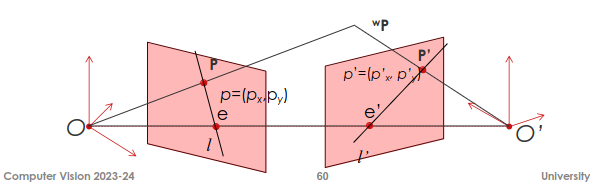
\includegraphics[width=0.65\textwidth]{Figures/found.png}
    % \caption{The world is the shared information.}
    \label{fig:found}
\end{figure}

But what does it represent? \\
For the moment we know the intrinsic parameters of the camera, this means that everything consists of roto-translations between cameras. In this case what we can say is that if we start from a \({}^WP\) what we have to understand is transformation that brings the coordinate system of one camera into the other, and this can be seen as a rotation and a translation:

\[
    Op\cdot[OO'\times O'p'] = 0
\]

What we are doing here is taking the vector that connects the two origins of the systems \(OO'\) and, by multiplication, bringing the vector \(O'p'\) into the other coordinate system. If the dot product between \(Op\) and the transformed \(O'p'\) is zero, it means that we actually have the match.

\begin{figure}[H]
\[
    Op\cdot[OO'\times O'p'] = 0 \;\;\;
    p\cdot[t\times Rp'] = 0 \;\;\;
    p = (u,v,1)^T \;\;\;
    p' = (u',v',1)^T \;\;\;
    p^T[t\times R]p'=0 \;\;\;
    p^TEp'=0    
\]
\caption{\textit{"You don't need to understand this"}- cit}
\label{eq:ess}
\end{figure}

After the transformations shown in \ref{eq:ess} we can map the two points with a single \textbf{Essential Matrix \(E\)}. This expression says that the matching between the two views is visible through a rotation and a translation of the origins. At this stage the \textbf{essential matrix} contains only the extrinsic information because, as we said, the intrinsic parameters are already known. %TODO: not sure about this one chief.. "are already known" ??

But we know that we have to deal with also the intrinsic parameters, fortunately it's nothing but a matrix to be added to the system.

\[
    p = K\hat{p} \;\;\;
    p' = K'\hat{p}' \;\;\;
    \rightarrow \;\;\;\;\;\; 
    F= K^{-T}EK'^{-1}
\]

In this way the point we obtain through se essential can be mapped using another transformation, \(K\) and \(K'\), and by combining the two we finally obtain the \textbf{fundamental matrix}. The foundamental matrix contains the roto-translation (the extrinsic) and also the instrinsic information. We can say that \(p\) and \(p'\) correspond as they are different projections of the same point in the two views. So, for each point \(p\) in one view, there's a corresponding epipolar
line \(l'\) in the other image.
\\
\\
Now that we have understood that we can go back to this expression, \(p' {}^TFp=0\). We use the world as shared information to find the correspondences, but once we have computed the matrix we have found the relationship between the points in the two image planes: we looked at the world to understand where the matches occurred, but now we can "forget" about it because we have a relationship that binds the two cameras.
\\
\\
The fundamental matrix is great because it gives the chance of determining the configuration of a system regardless of what are the coordinates in the real world, it means if we (rigidly) change the coordinates of the cameras in the real world, the same F will hold.
\\
\\
The camera matrices \({}^1M\) and \({}^2M\) are used to determine a \textit{unique} Fundamental Matrix \(F\) and while \({}^1M\) and \({}^2M\) are affected by rigid movements in the real world and \(F\) is not, on the other hand from a matrix \(F\) we can determine the camera matrices only to \textit{up a multiplication factor} of a certain matrix \(H\).

Given a fundamental matrix \(F\) for an object it's impossible to determine the absolute position in the world, the orientation and the scale. 
However, up to a projective transformation, the ambiguity in reconstruction can be solved, the projected points don't change if
\(
    MP = (MH^{-1})(HP)    
\)
\\
Where \(H\) is a projective transformation that does not affect the projection of \({}^WP\) onto the image plane.

\section{Homography and friends}

The planar homography \(H\) is a transformation that helps us make the mapping in between two planes that live in different domain. 

\begin{figure}[H]
    \centering
    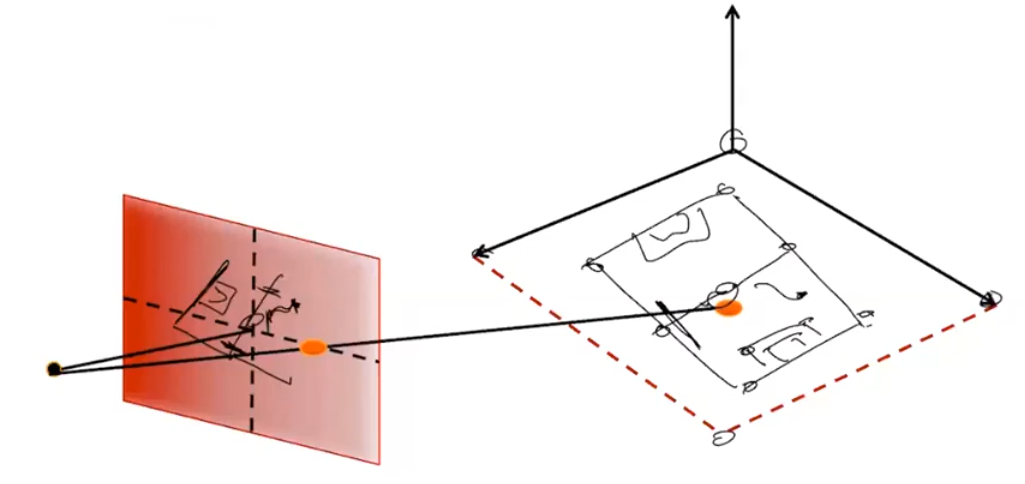
\includegraphics[width=0.65\textwidth]{Figures/homo.png}
    \caption{The planar homography.}
    \label{fig:homo}
\end{figure}

In Figure \ref{fig:homo} we can see how we are mapping a ground plane on the image plane, they are roto-translated and scaled by certain transformation, but we want to match these two planes in order to understand how things can be transferred from one domain to the other. This is the point where we go back to the real world.
\\
We have the fundamental matrix that deals with the camera configuration and we use the homography information to bind the views with the real world, we are talking about planes so, in the same way as we did before, what we do is to grab some \textbf{control points}, easily seen by both planes, such that if we know how this transformation occurs we can determine the correspondence of a displacement in the image plane to the displacement in the real plane. We can know that a displacement of 5px corresponds to a displacement of 3m in the real world thanks to the Homography Matrix \(H\).
\\\\
This is the basic element in order to determine the trajectory of something that moves on the ground plane, the process is the following:
\begin{itemize}
    \item Calibrate the cameras in a way that we are rectifying the distortion
    \item Determine the fundamental matrix, so where two points correspond in one view and in the other
    \item Take a reference on the real world, once we have that any movement in the image plane can be mapped to the real plane and can be converted in real coordinates.
\end{itemize}

In principle, we could do this even with a single camera, and we could use the second view to solve problems as occlusion. 

\subsection{2D Homography}

It's an invertible transformation between two planes, in fact in our first computation we try to match what is in the real world with what is in the image plane, once we have that we can track the movement in the image plane and we can convert it to the real world. The Homography matrix defined as \(H\) is the one that satisfies the following equation:
\[
    p' = Hp    
\]

Where \(p\) is a point in the world ground plane and \(p'\) is the corresponding point in the image plane. Since any vector crossed with itself gives 0 we can rewrite is as:

\[
    p' \times Hp = 0    
\]

We rely on this constraint in order to compute the matrix \(H\).

\begin{multicols}{2}
    

\[
    p' =
    \begin{bmatrix}
        x' \\
        y' \\
        1
    \end{bmatrix}
    =
    H
    \begin{bmatrix}
        x \\
        y \\
        1
    \end{bmatrix}
\]

\[
    p'= Hp
\]
\[
    p' \times Hp = 0
\]
\end{multicols}

We want to find a linear solution for \(H\), we can rewrite the vector \(Hp\) as:

\[
    Hp = 
    \begin{pmatrix}
        h^{1T}p\\
        h^{2T}p\\
        h^{3T}p
    \end{pmatrix}
\]

Now we want to compute the cross product, which is given as follows:

\[
    \begin{bmatrix}
        \hat{i} & \hat{j} & \hat{k} \\
        x' & y' & w' \\
        h^{1T}p & h^{2T}p & h^{3T}p
    \end{bmatrix}    
    =
    \begin{bmatrix}
        y'h^{3T}p - w'h^{2T}p \\
        -x'h^{3T}p + w'h^{1T}p \\
        x'h^{2T}p - y'h^{1T}p
    \end{bmatrix}
\]

And that's the result of the cross product, we can now rewrite the equation as a function of the components of \(H\):

\[
    \begin{bmatrix}
        0 & -w'p & y'p \\
        w'p & 0 & -x'p \\
        -y'p & x'p & 0
    \end{bmatrix}  
    \begin{bmatrix}
        h^{1T} \\
        h^{2T} \\
        h^{3T}
    \end{bmatrix}  
\]

At this point we know what's in the first matrix because we know the point in the second plane, we know the coordinates of the point in the first image plane \(P\) because we are matching coordinates, now our goal is to find the unknowns for \(H\).
Only two out of the 3 equations are independent, so one can be discarded, what we get in the end is a \(2\times 9\) matrix for which we need to determine the coefficients \(h\).

\[
    \begin{bmatrix}
        0 & -w'p & y'p \\
        w'p & 0 & -x'p \\
    \end{bmatrix}  
    \begin{bmatrix}
        h^{1T} \\
        h^{2T} \\
        h^{3T}
    \end{bmatrix}  
\]
For each matching point we have two equations, playing around with the number of points that we take we can solve the matrix, 4 points yield to the minimum number of equations to solve the system, but the more points we take the more robust the solution will be. The implementation available in OpenCV relies on the DLT, but otherwise we can use the regular Least-Squares approach.
\\
\\
We managed  to set up two cameras, link them to the real world thanks to the Homography matrix in such a way that we are able to determine the position of the object even in the case it's occluded. This is a very effective solution, we are only looking at the ground plane, not at the depth map, these solutions tend to be more robust and less noisy. It depends of course on the specific problem if it's needed or not to get the entire information about the scene depth.

\subsection{Multiple view geometry}

With multiple, we are referring to more than two. So far we have seen stereo systems with two cameras but of course we can generalize to an arbitrary number of views, this might be required in the case we need, for instance, a detailed point cloud. In this case we would end up in the area of so-called \textbf{voxels} with respect to pixels, small volume elements instead of screen elements.

\begin{figure}[H]
    \centering
    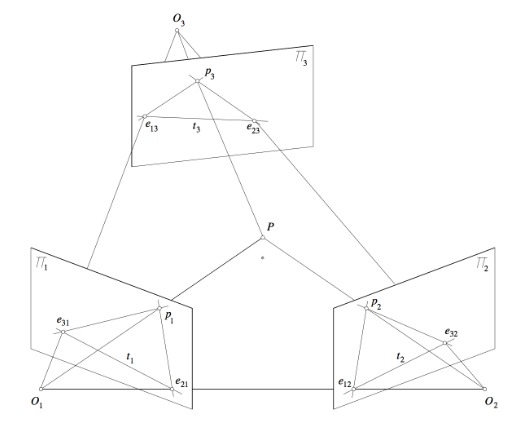
\includegraphics[scale=0.35]{Figures/multiv.png}
    \caption{Even in this case we can scale down to a two camera problem.}
    \label{fig:multiv}
\end{figure}

In Figure \ref{fig:multiv} can see how the point \({}^WP\) is being observed by the 3 cameras with projections \(P_1, P_2, P_3\). However, we know that these cameras can be linked together with epipolar geometry, provided some parameters of the cameras we should be able to determine the position of \({}^WP\) even with just two of them, and the same can be said for any two cameras. This system can be constructed as a combination of pairs of cameras, in this way the geometry constraints are fullfilled and using the essential matrix (or the fundamental matrix if we consider the intrinsic parameters) we can determine the position of the point in the real world and define the epipolar constraint as:
\[
    p^T_1E_{12}p_2=0
\]
\[
    p^T_2E_{23}p_3=0
\]
\[
    p^T_3E_{31}p_1=0
\]


At the end we can use any of the two equations to determine the position of the point in the real world, for instance we could use Camera 1 and Camera 2 in the case Camera 3 is occluded, sharing all these elements make it possible to come up with a very robust tracker. All this scales up to what we call the \textbf{problem of transfer}: make the network communicate in a way that the information is actually shared between the different cameras.
